\documentclass[conference,a4paper]{IEEEtran}
\usepackage{cite}
\usepackage{amsmath,amssymb}
\usepackage{graphicx}
\graphicspath{{assets/}{./}}
\usepackage{booktabs}
\usepackage{balance}
\usepackage{tikz}
\usetikzlibrary{arrows.meta,positioning}
\usepackage[hidelinks]{hyperref}

\begin{document}
\title{A Web-Based IoT Framework for Outflow-Tract Arrhythmia Localization Using a Compact 1D CNN Ensemble}
\author{
\IEEEauthorblockN{Daniandra Prayudisty Ilham}
\IEEEauthorblockA{\textit{Informatics, School of Computing}\\
\textit{Telkom University}\\Bandung 40257, Indonesia\\
daniandraaa@student.telkomuniversity.ac.id}
\and
\IEEEauthorblockN{Satria Mandala}
\IEEEauthorblockA{\textit{Humic Engineering, School of Computing}\\
\textit{Telkom University}\\Bandung 40257, Indonesia\\
satriamandala@telkomuniversity.ac.id}}
\maketitle

\begin{abstract}
Translating an electrocardiogram (ECG) classifier into a connected application requires preservation of signal processing, patient-level aggregation, and model provenance. This paper presents a web-based Internet of Things (IoT) gateway framework for left/right ventricular outflow-tract (LVOT/RVOT) origin localization from 12-lead ECG. A compact one-dimensional convolutional neural network (1D CNN; 170,914 parameters per model) is compared with a Random Forest (RF) using 132 morphology and RR-interval features. The frozen study cohort contains 289 patients from a public 334-patient database. On 230 development patients, five fixed patient-level folds evaluated with three initialization seeds produced macro-F1 scores of 0.9034$\pm$0.0285 for the CNN and 0.7753$\pm$0.0815 for RF; accuracies were 0.9278 and 0.8420. These are non-nested, configuration-selected results. Five-model ensembles achieved macro-F1 values of 0.8285 and 0.7209 on a previously inspected 59-patient historical hold-out. Replaying all 59 raw recordings through a sequenced HTTP/JSON gateway reproduced every offline class prediction for both models. Median CNN and RF pipeline times were 92.3 and 146.0~ms per record, respectively, while their 95th percentiles were 2370.6 and 254.4~ms. Five additional acquisition-paced replays returned both predictions a median of 264~ms after the finish request. The results support functional integration and a favorable CNN median-time tradeoff in this local workload; physical acquisition, wireless operation, and external clinical generalization remain untested.
\end{abstract}
\begin{IEEEkeywords}
Internet of Things, 12-lead ECG, ventricular arrhythmia, outflow-tract localization, convolutional neural network, Random Forest
\end{IEEEkeywords}

\section{Introduction}
Localization of an idiopathic ventricular arrhythmia to the left or right ventricular outflow tract (LVOT or RVOT) is a distinct task from identifying an abnormal beat. The former estimates an anatomical origin from the 12-lead electrocardiogram (ECG), whereas the latter identifies a rhythm or beat category. The public Ningbo database provides recordings of premature ventricular contractions (PVCs) and ventricular tachycardia (VT), with origin labels associated with successful ablation sites~\cite{zheng2020}. It offers a basis for developing automated origin-localization methods and studying how they can be integrated into a connected application.

Established ECG criteria include the V2 transition ratio~\cite{betensky2011} and the V2S/V3R index~\cite{yoshida2014}. These criteria encode relationships between precordial morphologies. Machine learning can combine a larger feature set: Zheng \emph{et al.}~\cite{zheng2021} developed a multistage approach using ECG morphology features for LVOT/RVOT discrimination. Deep neural networks have also been investigated for ECG rhythm classification~\cite{hannun2019} and 12-lead diagnosis~\cite{ribeiro2020}. Those tasks motivate learned signal representations, but their reported performance cannot be transferred directly to anatomical origin localization.

A usable connected system also needs a defined path from incoming signals to the model. Lead ordering, units, filtering, scaling, window aggregation, and artifact versions must agree with the offline experiment. A dashboard alone does not establish that agreement. Similarly, a fast isolated forward pass does not measure the complete cost of preprocessing and inference. For an Internet of Things (IoT) application, a gateway interface and measurements across the communication-to-inference path provide more concrete integration evidence.

This work develops a web application and HTTP gateway around a compact CNN-only inference model, with a feature-based Random Forest (RF) comparator. Its scope is the application and the measured behavior of two frozen pipelines. The contributions are: (1) a sequenced, chunk-based interface for 12-lead ECG and record-level localization; (2) an explicitly qualified patient-level comparison of CNN and RF configurations; and (3) replay-based validation of prediction consistency and processing latency. The current gateway source is the actual public dataset, rather than a physical ECG acquisition device. This distinction defines what the experiments demonstrate.

\section{Related Work}
Betensky \emph{et al.}~\cite{betensky2011} and Yoshida \emph{et al.}~\cite{yoshida2014} proposed ECG indices that use precordial morphology to distinguish outflow-tract origins. Zheng \emph{et al.} released a 334-patient 12-lead database~\cite{zheng2020} and subsequently investigated feature extraction and machine learning for left/right origin classification~\cite{zheng2021}. Their feature-engineering strategy differs from the 132-feature RF implemented here. Consequently, the present RF is a reproducible local comparator, rather than a reproduction of that published classifier or a claim about the strongest available feature-based method.

Hannun \emph{et al.}~\cite{hannun2019} studied deep learning for ambulatory rhythm classification, and Ribeiro \emph{et al.}~\cite{ribeiro2020} studied automated 12-lead ECG diagnosis. In a related connected-system setting, Ardian and Mandala~\cite{ardian2025} integrated a modified Transformer decoder and conditional ECG-GAN into an IoT-oriented arrhythmia detection application. That study addresses beat classes; the present output is a binary LVOT/RVOT origin at recording level. We therefore evaluate origin discrimination and gateway consistency separately, without treating performance across these different targets and cohorts as directly comparable. The CNN architecture and conditional augmentation are established building blocks; the emphasis here is their integration and the measured CNN/RF tradeoff.

\section{Materials and Methods}
\subsection{Dataset, Cohort, and Evaluation Units}
The source database contains 334 subjects recorded at 2000~Hz~\cite{zheng2020}. The local diagnosis spreadsheet has a coarse left/right label for every subject. However, the frozen cohort inherited from earlier experiments was defined using its local \texttt{Sublocation} field: five Summit records were excluded, and 40 records lacked that field. Thus, the latter records do have coarse left/right labels; their exclusion reflects the earlier cohort definition, not absence of a binary origin in the public resource. We retain this fixed cohort to compare the existing model artifacts without changing the evaluation population after observing results.

The resulting 289-patient cohort contains 71 LVOT and 218 RVOT cases, including 286 PVC and three VT records. It is therefore described as ventricular arrhythmia origin localization, rather than exclusively PVC localization. Table~\ref{tab:cohort} gives the fixed partitions. The 59-patient partition was separated during prior work and has since been inspected in exploratory analyses. It is reported as a \emph{historical hold-out}, not as a new independent or external test. Development-set cross-validation (CV) is the principal descriptive comparison, with selection-related limitations stated below. Every split is by patient; overlapping windows from a patient never appear on both sides of a fold.

\begin{table}[t]
\caption{Frozen cohort and partition counts.}
\label{tab:cohort}\centering
\begin{tabular}{lrrr}\toprule
Partition & LVOT & RVOT & Total\\\midrule
Development & 57 & 173 & 230\\
Historical hold-out & 14 & 45 & 59\\\midrule
Included cohort & 71 & 218 & 289\\\bottomrule
\end{tabular}
\end{table}

\subsection{Canonical CNN Signal Processing}
The lead order is I, II, III, aVR, aVL, aVF, and V1--V6. Native dataset amplitudes and sampling frequency are preserved. The complete record is high-pass filtered with a fourth-order Butterworth filter at 0.5~Hz using forward--backward filtering. A level-five coif5 discrete wavelet transform applies level-wise SURE soft thresholding, following the wavelet-shrinkage principle~\cite{donoho1995}. Processing produces float32 values. These operations use the complete record and are noncausal.

The denoised signal is divided into 5000-point windows (2.5~s), with a 2500-point step. Only complete windows are used; an incomplete trailing window is discarded. Each lead is standardized using means and scales estimated exclusively from the training patients for that fold. Final deployment uses the scaler fitted on the 230 development patients. Whole-record filtering, window boundaries, and lead scaling are reused in the server rather than replaced with browser-side approximations.

\subsection{CNN Architecture and Patient Aggregation}
Four convolutional blocks use 32, 64, 128, and 256 channels, with respective kernel lengths 7, 5, 3, and 3. Each block contains same-padded convolution, batch normalization, ReLU, and factor-two max pooling. Global temporal averaging feeds a head consisting of layer normalization, a 256-to-128 linear layer, ReLU, dropout of 0.3, and a two-output linear layer. Each model has 170,914 trainable parameters; the five deployed CNNs therefore contain 854,570 trainable parameters in total. ``Compact'' describes the individual architecture's parameter count, rather than a measured energy or embedded-device advantage. The deployed predictor uses CNN blocks only; no Transformer is used at inference.

Let $p_{s,w}(c)$ denote the softmax probability for class $c$ from window $w$ and model seed $s$. With $W_i$ complete windows in patient $i$, its single-model probability is
\begin{equation}
\bar p_{i,s}(c)=\frac{1}{W_i}\sum_{w=1}^{W_i}p_{s,w}(c).
\label{eq:pool}
\end{equation}
For deployment, the five seeds $\{42,43,44,45,46\}$ are averaged:
\begin{equation}
\hat p_i(c)=\frac{1}{5}\sum_s\bar p_{i,s}(c).
\label{eq:ensemble}
\end{equation}
RVOT is assigned when $\hat p_i(\mathrm{RVOT})>0.5$; otherwise the result is LVOT. Probabilities are not calibrated risk estimates. The CV results below describe individual fitted models, whereas the historical hold-out and gateway results describe five-model ensembles.

\subsection{Training and Conditional Augmentation}
Training uses patient bags of up to four windows and a class-weighted patient negative log-likelihood after probability pooling. A conditional generative adversarial network (GAN)~\cite{mirza2014}, fitted only to the training patients of the corresponding fold, supplies class-matched synthetic windows. When a four-window bag is available, one window is replaced with a generated window. This is a training augmentation step: validation, historical hold-out, and gateway inference use only real ECG. The augmentation is retained in this description even though the deployed predictor itself is CNN-only.

The CNN setting was selected from a nine-point grid of learning rates $\{10^{-4},5\times10^{-4},10^{-3}\}$ and window batch budgets $\{16,32,64\}$ with augmentation, plus a no-augmentation baseline at $10^{-3}$ and 32. The selected setting uses $5\times10^{-4}$ and 16. AdamW has weight decay $10^{-4}$, cosine learning-rate decay to $10^{-6}$ over at most 100 epochs, gradient clipping at 1.0, and early stopping with patience 15 using validation macro-F1. No pretrained weights are used. The final five CNN models were fitted on all development patients for the selected 16 epochs. Their augmentation generator was fitted on the development partition only.

\subsection{Random Forest Comparator}
The RF~\cite{breiman2001} uses 132 morphology and RR-interval features measured from the full raw recording by a separate beat-delineation pipeline. Per-lead descriptors include QRS width, relative R and S amplitudes, R fraction, and signed QRS area. Global descriptors include robust QRS span, precordial transition, V2S/V3R, and three RR measurements. The median and interquartile range over detected beats form the fixed feature vector. Missing features are median-imputed using training-patient values only.

Each forest has 500 trees, balanced class weights, and otherwise default scikit-learn settings. The RF was not hyperparameter-tuned and does not use GAN augmentation. It uses the same patient folds and initialization seeds as the CNN; final deployment averages five forest probabilities. This comparison therefore concerns the two implemented pipelines, including their training choices. It does not isolate architecture from augmentation and tuning effort.

\subsection{Metrics and Exploratory Uncertainty}
Five fixed stratified folds on 230 patients are evaluated with three initialization seeds, 42--44, giving 15 fits per model. The fold partitions do not change with the initialization seed. Reported means and standard deviations summarize those fits; they are not results from 15 independent patient cohorts. The primary descriptive metric is macro-F1, the unweighted mean of class-specific F1 scores. Accuracy, balanced accuracy, LVOT/RVOT sensitivity, and ROC AUC based on RVOT probability provide complementary measures for the imbalanced cohort.

For paired macro-F1 differences $d_j$ across the 15 fold/seed fits, an approximate corrected standard error is
\begin{equation}
\operatorname{SE}_{\mathrm{corr}}=\sqrt{\left(\frac{1}{15}+\frac{46}{184}\right)s_d^2},
\label{eq:se}
\end{equation}
with a $t_{14}$ reference, following the dependence correction of Nadeau and Bengio~\cite{nadeau2003}. The approximation acknowledges overlapping training sets but does not make the fixed-fold seed results independent. More importantly, the same CV results were used to select the CNN setting. Intervals and $p$-values are therefore exploratory and not adjusted for configuration selection; nested CV is needed for a less selection-biased estimate. Historical hold-out ensemble differences use a paired, class-stratified bootstrap with 5000 resamples and an exact McNemar test~\cite{mcnemar1947}. Prior inspection also limits interpretation of those intervals.

\section{Gateway and Web Application}
\subsection{Record Transfer and Inference}
Fig.~\ref{fig:system} places ECG acquisition upstream of the IoT gateway, preprocessing, inference, and user interface. In the target acquisition path, electrodes and a 12-lead ECG device capture and digitize the patient signal; the gateway transports the resulting record to the server. ECG acquisition supplies the signal, while the CNN performs anatomical origin localization. In this study, real recordings from the public database are injected at the same gateway boundary to evaluate the downstream application. The physical device interface and live acquisition have not been characterized in these experiments. A Python gateway reads a real 12-lead dataset file and opens an HTTP/JSON session containing sampling rate, lead order, amplitude-unit metadata, and expected recording length. Chunks contain a sequence number, sample offset, and a matrix of ECG values. The server supports up to 8000 time points per chunk. An identical retransmission is handled idempotently; a gap, conflicting retransmission, or inconsistent offset is rejected. Finalization checks completeness before running the inference pipelines.

\begin{figure*}[t]
\centering
\resizebox{\textwidth}{!}{%
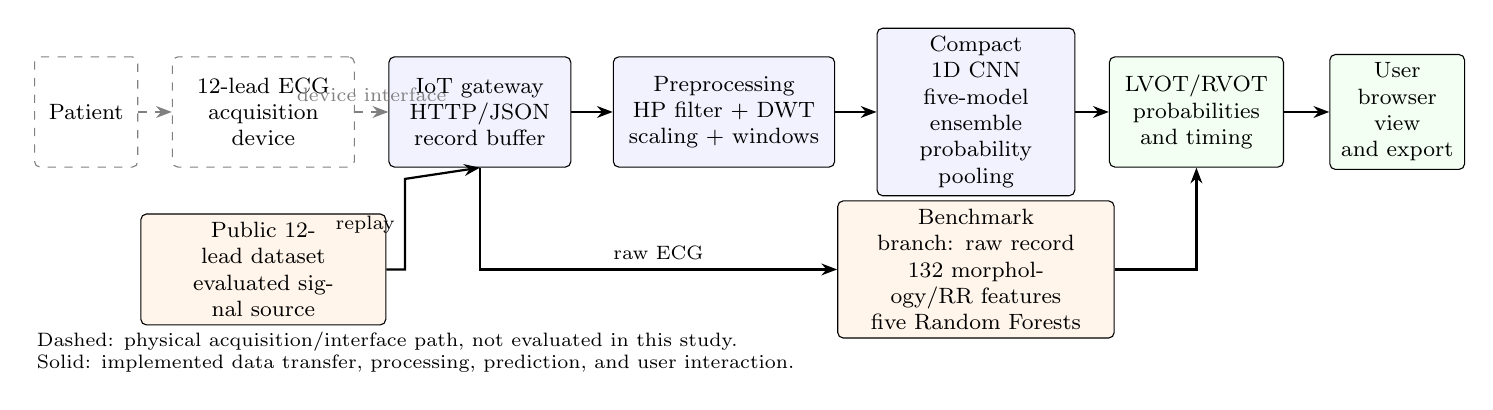
\begin{tikzpicture}[font=\footnotesize,
 box/.style={draw,rounded corners=2pt,align=center,minimum height=14mm,inner sep=3pt},
 arr/.style={-{Stealth[length=2mm]},thick},
 target/.style={arr,dashed,gray}]
\node[box,text width=11mm,dashed,draw=gray] (patient) at (0,0) {Patient};
\node[box,text width=21mm,dashed,draw=gray] (device) at (2.25,0) {12-lead ECG\\acquisition\\device};
\node[box,text width=21mm,fill=blue!5] (gateway) at (5.0,0) {IoT gateway\\HTTP/JSON\\record buffer};
\node[box,text width=26mm,fill=blue!5] (pre) at (8.1,0) {Preprocessing\\HP filter + DWT\\scaling + windows};
\node[box,text width=23mm,fill=blue!5] (cnn) at (11.3,0) {Compact 1D CNN\\five-model ensemble\\probability pooling};
\node[box,text width=20mm,fill=green!5] (output) at (14.1,0) {LVOT/RVOT\\probabilities\\and timing};
\node[box,text width=15mm,fill=green!5] (user) at (16.65,0) {User\\browser view\\and export};
\node[box,text width=29mm,fill=orange!8] (dataset) at (2.25,-2.0) {Public 12-lead dataset\\evaluated signal source};
\node[box,text width=33mm,fill=orange!8] (rf) at (11.3,-2.0) {Benchmark branch: raw record\\132 morphology/RR features\\five Random Forests};
\draw[target] (patient)--(device);
\draw[target] (device)--node[above,font=\scriptsize]{device interface}(gateway);
\draw[arr] (gateway)--(pre);
\draw[arr] (pre)--(cnn);
\draw[arr] (cnn)--(output);
\draw[arr] (output)--(user);
\draw[arr] (dataset.east)--(4.05,-2.0)--node[left,font=\scriptsize]{replay}(4.05,-.85)--(gateway.south);
\draw[arr] (gateway.south)--(5.0,-2.0)--node[above,font=\scriptsize]{raw ECG}(rf.west);
\draw[arr] (rf.east)-|(output.south);
\node[align=left,font=\scriptsize,anchor=west] at (-.75,-3.05) {Dashed: physical acquisition/interface path, not evaluated in this study.\\Solid: implemented data transfer, processing, prediction, and user interaction.};
\end{tikzpicture}}
\caption{Acquisition-to-user architecture. A physical ECG device is the intended upstream signal source for the IoT gateway. The completed experiments inject real public-dataset recordings at the gateway and evaluate the solid paths. Device output format, live capture, and wireless transport are outside the measured scope. The RF branch receives the raw record and performs its own feature processing.}
\label{fig:system}
\end{figure*}

The Python server uses PyTorch for CNN inference, scikit-learn for RF, and a browser-based dashboard. Both predictions, class probabilities, waveform previews, and stage timings are returned through the application. The catalog exposes all 334 source records while distinguishing the 289 supported cohort entries from the excluded entries. Catalog visibility is separate from the number of patients used to train or evaluate a model. The application also distinguishes the frozen CV summary from the historical hold-out summary; displaying a CV macro-F1 of approximately 0.90 does not make that value the accuracy of an individual gateway prediction.

The CNN checkpoints and scaler are verified against their recorded SHA-256 provenance at startup; RF artifact hashes are recorded as part of the deployed artifact identity. Session summaries retain results and timing without storing the full raw waveform. The interface supports bearer-token access when serving a local network. Authentication capability is not evidence of an evaluated production security deployment: the experiments here use loopback HTTP, and do not measure encrypted wireless transfer or remote operation.

\subsection{Web Interface and Implementation Evidence}
Fig.~\ref{fig:webapp} documents the running application using an actual historical hold-out recording, ECG-231. The interface displays all 12 received leads, the completed acquisition status, and a record-level RVOT output with a CNN probability of 98.0\% and RF probability of 82.2\%. These are rounded model outputs for one recording, rather than estimates of diagnostic accuracy. The heart graphic is a schematic orientation cue, not a reconstructed patient-specific anatomical map. A separate CV summary panel displays the fixed 230-patient evaluation, so population metrics remain distinguishable from the selected record's prediction.

The user workflow is to select or upload a record, start transfer, inspect the received waveform, and review the final localization after preprocessing and inference. The dashboard also exposes stage timings, session history, and result export. The screenshots substantiate an implemented user interface; end-to-end replay and automated functional checks provide separate evidence that its server path executes the frozen models.

\begin{figure*}[t]
\centering
\begin{minipage}[t]{0.63\textwidth}
\centering
{\footnotesize\textbf{(a) Received 12-lead ECG and completed transfer}}\\[2pt]
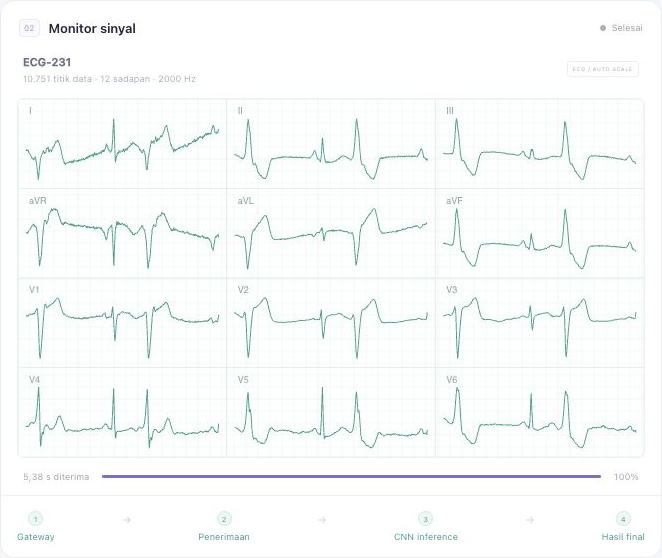
\includegraphics[width=\linewidth]{web_signal.png}\\[5pt]
{\footnotesize\textbf{(c) Separate development-CV summary}}\\[2pt]

\includegraphics[width=\linewidth]{web_cv_summary.png}
\end{minipage}\hfill
\begin{minipage}[t]{0.34\textwidth}
\centering
{\footnotesize\textbf{(b) Record-level localization output}}\\[2pt]
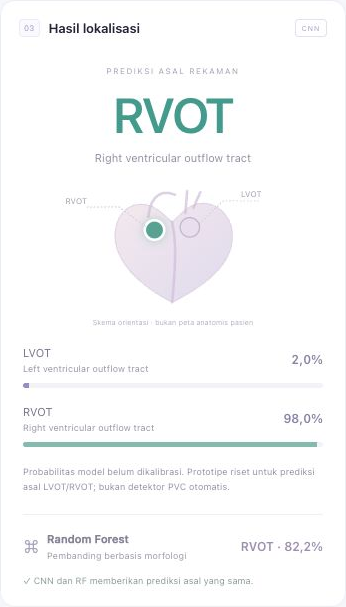
\includegraphics[width=\linewidth]{web_result.png}
\end{minipage}
\caption{Cropped screenshots from the functioning web application. Panels (a) and (b) show ECG-231 (5.3755~s, 12 leads, 2000~Hz) replayed from the historical hold-out at acquisition pace. Panel (c) shows the separate selected-configuration CV summary (230 patients; five fixed folds and three initialization seeds). Screenshot values use Indonesian decimal commas. The interface images show implemented behavior on public ECG data and do not establish live physical-device acquisition.}
\label{fig:webapp}
\end{figure*}

\subsection{System Evaluation Protocol}
All 59 historical hold-out raw records were transmitted through the gateway in 1000-time-point chunks, equivalent to 0.5~s of signal per full chunk. One warm-up replay was excluded. The principal run sends chunks without acquisition delays, once per record. A second run replays the first five records at 2000 time points/s. These five repeated records are system tests, not additional diagnostic subjects. The client and server run on the same Apple Silicon arm64 workstation with macOS 26.2, PyTorch 2.12.0, CPU inference, and four PyTorch threads. RF prediction uses one job per forest. The deployed identity is \texttt{154da12ade375dff}, using seeds 42--46.

For each record, CNN pipeline time is preprocessing plus inference by the five CNN models. RF pipeline time is feature extraction plus inference by the five forests. Their distributions are computed from these per-record sums, rather than by adding marginal stage medians. The finish-request round trip measures the final request and response, including processing both models. Client end-to-end time also includes session creation, chunk serialization and transfer, and, for paced replays, acquisition waiting. These definitions prevent acquisition time from being confused with model inference time.

\section{Results}
\subsection{Development-Set Comparison}
Table~\ref{tab:cv} reports the 15-fit summaries. CNN macro-F1 is 0.9034 compared with 0.7753 for RF, with a mean paired difference of 0.1281. The exploratory corrected 95\% interval is [0.0247, 0.2314], with $p=0.0188$. CNN has higher macro-F1 in 13 fits and ties in two. Fig.~\ref{fig:cv} shows the paired results rather than treating the aggregate mean as a result attained identically by every fit.

\begin{table}[t]
\caption{Development CV: mean $\pm$ SD over five fixed patient folds and three initialization seeds. Selection was not nested.}
\label{tab:cv}\centering\small
\begin{tabular}{lcc}\toprule
Metric & 1D CNN & Random Forest\\\midrule
Macro-F1 & $0.9034\pm0.0285$ & $0.7753\pm0.0815$\\
ROC AUC & $0.9349\pm0.0260$ & $0.8510\pm0.0768$\\
Accuracy & $0.9278\pm0.0217$ & $0.8420\pm0.0561$\\
Balanced accuracy & $0.9045\pm0.0340$ & $0.7673\pm0.0865$\\
LVOT sensitivity & $0.8591\pm0.0779$ & $0.6197\pm0.1737$\\
RVOT sensitivity & $0.9500\pm0.0300$ & $0.9148\pm0.0607$\\\bottomrule
\end{tabular}
\end{table}
\begin{figure}[t]\centering
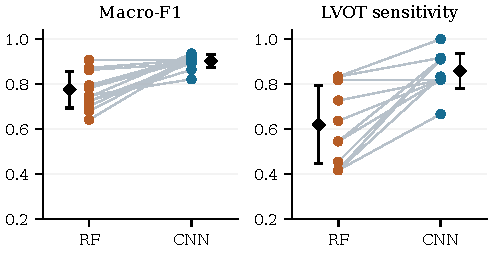
\includegraphics[width=\columnwidth]{cv_paired.pdf}
\caption{Paired fold/seed results. Lines join matched fits; black diamonds and bars denote means and SDs. Shared patients and folds limit independence.}
\label{fig:cv}
\end{figure}

The larger descriptive difference occurs in LVOT sensitivity: 0.8591 for CNN compared with 0.6197 for RF. RVOT sensitivity remains 0.9500 and 0.9148, respectively. Thus, accuracy alone would understate the RF's minority-class errors. CNN macro-F1 also varies less across these fits (SD 0.0285 compared with 0.0815). The mean AUC difference is 0.0839, but its exploratory corrected interval includes zero ([$-0.0241$, 0.1920]). These results support describing the observed configuration comparison without asserting a selection-adjusted statistical superiority claim.

\subsection{Historical Hold-Out Ensembles}
Table~\ref{tab:holdout} and Fig.~\ref{fig:cm} summarize the five-model ensembles on 59 patients. CNN correctly classifies 12 of 14 LVOT and 39 of 45 RVOT cases; RF correctly classifies seven LVOT and 41 RVOT cases. The higher CNN minority-class sensitivity accompanies two fewer correct RVOT classifications, rather than improvement for every class and patient.

\begin{table}[t]
\caption{Historical hold-out: 59 patients, including 14 LVOT. Values describe five-seed ensembles, unless indicated.}
\label{tab:holdout}\centering\small
\setlength{\tabcolsep}{4pt}
\begin{tabular}{lcc}\toprule
Metric & 1D CNN & Random Forest\\\midrule
Macro-F1 & 0.8285 & 0.7209\\
ROC AUC & 0.9413 & 0.7413\\
Accuracy & 0.8644 & 0.8136\\
Balanced accuracy & 0.8619 & 0.7056\\
LVOT sensitivity & 0.8571 & 0.5000\\
RVOT sensitivity & 0.8667 & 0.9111\\
Single-model F1$^{*}$ & $0.7930\pm0.0382$ & $0.7144\pm0.0192$\\\bottomrule
\end{tabular}
\\[2pt]{\footnotesize $^{*}$Mean$\pm$SD across five individual models.}
\end{table}
\begin{figure}[t]\centering
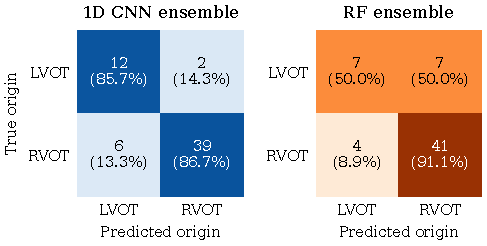
\includegraphics[width=\columnwidth]{holdout_confusion.pdf}
\caption{Historical hold-out confusion matrices. Counts are accompanied by within-row percentages; neither matrix represents an external validation cohort.}
\label{fig:cm}
\end{figure}

The paired macro-F1 difference is 0.1076, with a bootstrap 95\% interval of [$-0.0263$, 0.2568]. Seven patients are correct only with CNN, and four only with RF; exact McNemar $p=0.5488$. The AUC difference is 0.2000, with interval [0.0667, 0.3492]. The macro-F1 interval includes zero, and only 14 LVOT patients are available. These small, previously inspected data do not establish an independent confirmatory advantage. The lower hold-out F1 than development CV also illustrates why 0.9034 must be presented specifically as a selected-configuration CV mean.

\subsection{Gateway Prediction Consistency}
All 59 no-delay replays complete successfully. Source durations range from 5.053 to 25.000~s, with a median of 12.943~s. Gateway and offline class predictions agree for 59/59 recordings for each model. The maximum absolute RVOT probability discrepancy is $2.51\times10^{-7}$ for CNN and zero for RF. All five acquisition-paced replays also preserve both class predictions. These results validate consistency of record transfer, canonical processing, and probability aggregation for the evaluated records. The 100\% agreement is an implementation-consistency measure; diagnostic accuracies remain 0.8644 and 0.8136, respectively.

\subsection{Application Functional Verification}
Eleven automated application tests exercise the real HTTP server and frozen model artifacts. Table~\ref{tab:functional} summarizes representative checks. The suite covers valid transfer, input rejection, duplicate handling, prediction parity, result persistence, cohort accounting, and measured-efficiency export. These checks assess software behavior; neither a passing test nor a screenshot adds new diagnostic patients or validates a physical ECG device.

\begin{table}[t]
\caption{Representative application checks from the 11-test suite.}
\label{tab:functional}\centering\small
\setlength{\tabcolsep}{3pt}
\begin{tabular}{p{.34\columnwidth}p{.46\columnwidth}c}\toprule
Check & Expected behavior & Result\\\midrule
Complete HTTP record & Finalize; preserve offline prediction & Pass\\
Identical chunk retry & Accept once; no duplicated points & Pass\\
Gap/conflicting chunk & Reject; preserve ordered buffer & Pass\\
Incomplete record & Reject finalization & Pass\\
Wrong rate/leads/unit & Reject incompatible model input & Pass\\
Result export & Persist predictions, timing, provenance & Pass\\\bottomrule
\end{tabular}
\end{table}

\subsection{Processing Time and Transfer Behavior}
Table~\ref{tab:latency} reports timing for the 59 no-delay replays. Median CNN pipeline processing is 92.3~ms per record compared with 146.0~ms for RF, a ratio of approximately 1.6. However, the CNN has a substantially longer tail: its P95 is 2370.6~ms compared with 254.4~ms for RF. Fig.~\ref{fig:latency} displays the complete empirical distributions. The median supports a favorable CNN tradeoff in this workload; the tail prevents a claim of uniformly faster or deterministic real-time inference.

\begin{table}[t]
\caption{Local no-delay gateway timing over 59 recordings (ms per record). Pipeline percentiles use per-record stage sums.}
\label{tab:latency}\centering\small
\begin{tabular}{lrr}\toprule
Stage & Median & P95\\\midrule
CNN preprocessing & 34.2 & 68.9\\
CNN inference, five models & 57.0 & 2310.2\\
\textbf{CNN pipeline} & \textbf{92.3} & \textbf{2370.6}\\
RF feature extraction & 47.0 & 109.0\\
RF inference, five forests & 94.7 & 163.4\\
\textbf{RF pipeline} & \textbf{146.0} & \textbf{254.4}\\\midrule
Server processing, both models & 239.6 & 2525.3\\
Finish-request round trip & 245.3 & 2530.8\\
Client end-to-end, no delay & 551.6 & 3032.5\\\bottomrule
\end{tabular}
\end{table}
\begin{figure}[t]\centering
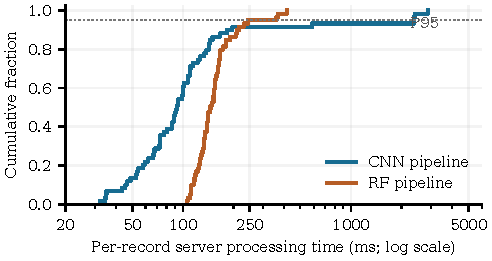
\includegraphics[width=\columnwidth]{latency_ecdf.pdf}
\caption{Empirical cumulative pipeline-time distributions for 59 local replays. The logarithmic time axis exposes the CNN tail; the dotted line marks a cumulative fraction of 0.95.}
\label{fig:latency}
\end{figure}

The median across per-record median chunk round trips is 10.2~ms for chunks representing 500~ms of acquisition. For the five acquisition-paced records, both-model finish-request round trips have median 264~ms and maximum 427~ms. The largest within-record chunk P95 in that paced subset is 51.6~ms, below its 500~ms acquisition interval. This shows the implemented local transfer path keeping pace for those five records. It does not characterize wireless delays, packet loss, concurrent clients, or an unmeasured acquisition device. Because full-record noncausal processing precedes localization, the measured response is a post-acquisition record result, not continuous PVC detection.

\section{Discussion and Limitations}
The application connects frozen offline classifiers to an explicit gateway protocol and exposes both diagnostic and operational measurements. A practical strength is reproducibility of the same patient-level decision after chunked transfer. Small probability discrepancies without label changes are consistent with floating-point execution differences. Reporting artifact identity, cohort boundaries, and the evaluation unit makes the displayed performance traceable to an experiment rather than to an arbitrary dashboard value.

The CNN has higher observed macro-F1 and LVOT sensitivity in the selected CV configuration. Learned morphology may capture information omitted by the fixed feature extractor, but this experiment does not establish that mechanism. CNN tuning and conditional augmentation differ from the untuned RF training. A tuned RF, alternative feature selection, matched augmentation, or nested selection could change the comparison. The earlier dataset study also uses a different engineered representation~\cite{zheng2021}; the current numbers should not be interpreted as a state-of-the-art ranking across papers.

Runtime has a similarly qualified interpretation. Avoiding explicit beat-feature extraction reduces one CNN preprocessing component, yet RF inference itself has a larger median cost than RF feature extraction. Feature extraction therefore does not dominate every RF stage. Conversely, the CNN latency tail is substantial. The single-pass, varying-duration workload lacks controlled background CPU load and repeated per-record trials; its measurements cannot attribute that tail to a particular scheduler or implementation component. Neither energy consumption nor edge-device execution was measured. The compact per-model parameter count alone does not prove efficiency of the full five-model deployment on an embedded device.

The data originate from one clinical center. The historical hold-out has been inspected previously, CV selection is non-nested, and initialization repetitions reuse the same patient folds. Excluding 40 records because of a local sublocation field despite available coarse labels also restricts representativeness. Reintegrating eligible records requires a prospectively specified cohort and fresh evaluation, rather than adding them only to the displayed patient count. The three retained VT records further prevent a PVC-only population claim.

Finally, physical acquisition, cross-device amplitude calibration, wireless transport, concurrency, calibrated confidence, and external validation remain open. The HTTP interface supplies an integration boundary for a future acquisition gateway, but loopback replay is the completed IoT-system evidence. A future study should freeze the cohort and preprocessing prospectively, compare equally tuned alternatives, evaluate a causal processing path if continuous output is required, and validate on an independently collected center/device cohort. The current application is a research system and has not been evaluated for clinical decision-making.

\balance
\section{Conclusion}
A web-based IoT gateway framework was implemented for record-level LVOT/RVOT origin localization using a compact CNN-only predictor and an RF comparator. The selected CNN configuration achieved development CV macro-F1 of 0.9034 compared with 0.7753 for RF; historical hold-out ensemble values were 0.8285 and 0.7209. All 59 gateway replays preserved offline class predictions. CNN median pipeline time was lower (92.3 compared with 146.0~ms), while its P95 was higher (2370.6 compared with 254.4~ms). The study supports functional integration and a measured local tradeoff, with independent predictive validation and physical IoT acquisition as necessary next steps.

\begin{thebibliography}{00}
\bibitem{zheng2020} J. Zheng, G. Fu, K. Anderson, H. Chu, and C. Rakovski, ``A 12-lead ECG database to identify origins of idiopathic ventricular arrhythmia containing 334 patients,'' \emph{Sci. Data}, vol. 7, Art. no. 98, 2020, doi: 10.1038/s41597-020-0440-8.
\bibitem{betensky2011} B. P. Betensky \emph{et al.}, ``The V2 transition ratio: A new electrocardiographic criterion for distinguishing left from right ventricular outflow tract tachycardia origin,'' \emph{J. Am. Coll. Cardiol.}, vol. 57, no. 22, pp. 2255--2262, 2011, doi: 10.1016/j.jacc.2011.01.035.
\bibitem{yoshida2014} N. Yoshida \emph{et al.}, ``A novel electrocardiographic criterion for differentiating a left from right ventricular outflow tract tachycardia origin: The V2S/V3R index,'' \emph{J. Cardiovasc. Electrophysiol.}, vol. 25, no. 7, pp. 747--753, 2014, doi: 10.1111/jce.12392.
\bibitem{zheng2021} J. Zheng \emph{et al.}, ``A high-precision machine learning algorithm to classify left and right outflow tract ventricular tachycardia,'' \emph{Front. Physiol.}, vol. 12, Art. no. 641066, 2021, doi: 10.3389/fphys.2021.641066.
\bibitem{hannun2019} A. Y. Hannun \emph{et al.}, ``Cardiologist-level arrhythmia detection and classification in ambulatory electrocardiograms using a deep neural network,'' \emph{Nat. Med.}, vol. 25, pp. 65--69, 2019, doi: 10.1038/s41591-018-0268-3.
\bibitem{ribeiro2020} A. H. Ribeiro \emph{et al.}, ``Automatic diagnosis of the 12-lead ECG using a deep neural network,'' \emph{Nat. Commun.}, vol. 11, Art. no. 1760, 2020, doi: 10.1038/s41467-020-15432-4.
\bibitem{ardian2025} M. N. T. Ardian and S. Mandala, ``IoT-enabled real-time arrhythmia detection using modified transformer decoder and conditional ECG-GAN,'' in \emph{Proc. IEEE AGERS}, 2025, pp. 204--211.
\bibitem{donoho1995} D. L. Donoho and I. M. Johnstone, ``Adapting to unknown smoothness via wavelet shrinkage,'' \emph{J. Am. Stat. Assoc.}, vol. 90, no. 432, pp. 1200--1224, 1995, doi: 10.1080/01621459.1995.10476626.
\bibitem{mirza2014} M. Mirza and S. Osindero, ``Conditional generative adversarial nets,'' arXiv:1411.1784, 2014.
\bibitem{breiman2001} L. Breiman, ``Random forests,'' \emph{Mach. Learn.}, vol. 45, pp. 5--32, 2001, doi: 10.1023/A:1010933404324.
\bibitem{nadeau2003} C. Nadeau and Y. Bengio, ``Inference for the generalization error,'' \emph{Mach. Learn.}, vol. 52, pp. 239--281, 2003, doi: 10.1023/A:1024068626366.
\bibitem{mcnemar1947} Q. McNemar, ``Note on the sampling error of the difference between correlated proportions or percentages,'' \emph{Psychometrika}, vol. 12, pp. 153--157, 1947, doi: 10.1007/BF02295996.
\end{thebibliography}
\end{document}
